\subsubsection{range\_check\_u32}

U32RangeCheckGate is a gate which can decompose a number into base B little-endian limbs.

Gate structure is like figure \ref{fig:range-check-u32}.

\begin{figure}[!ht]
    \centering
    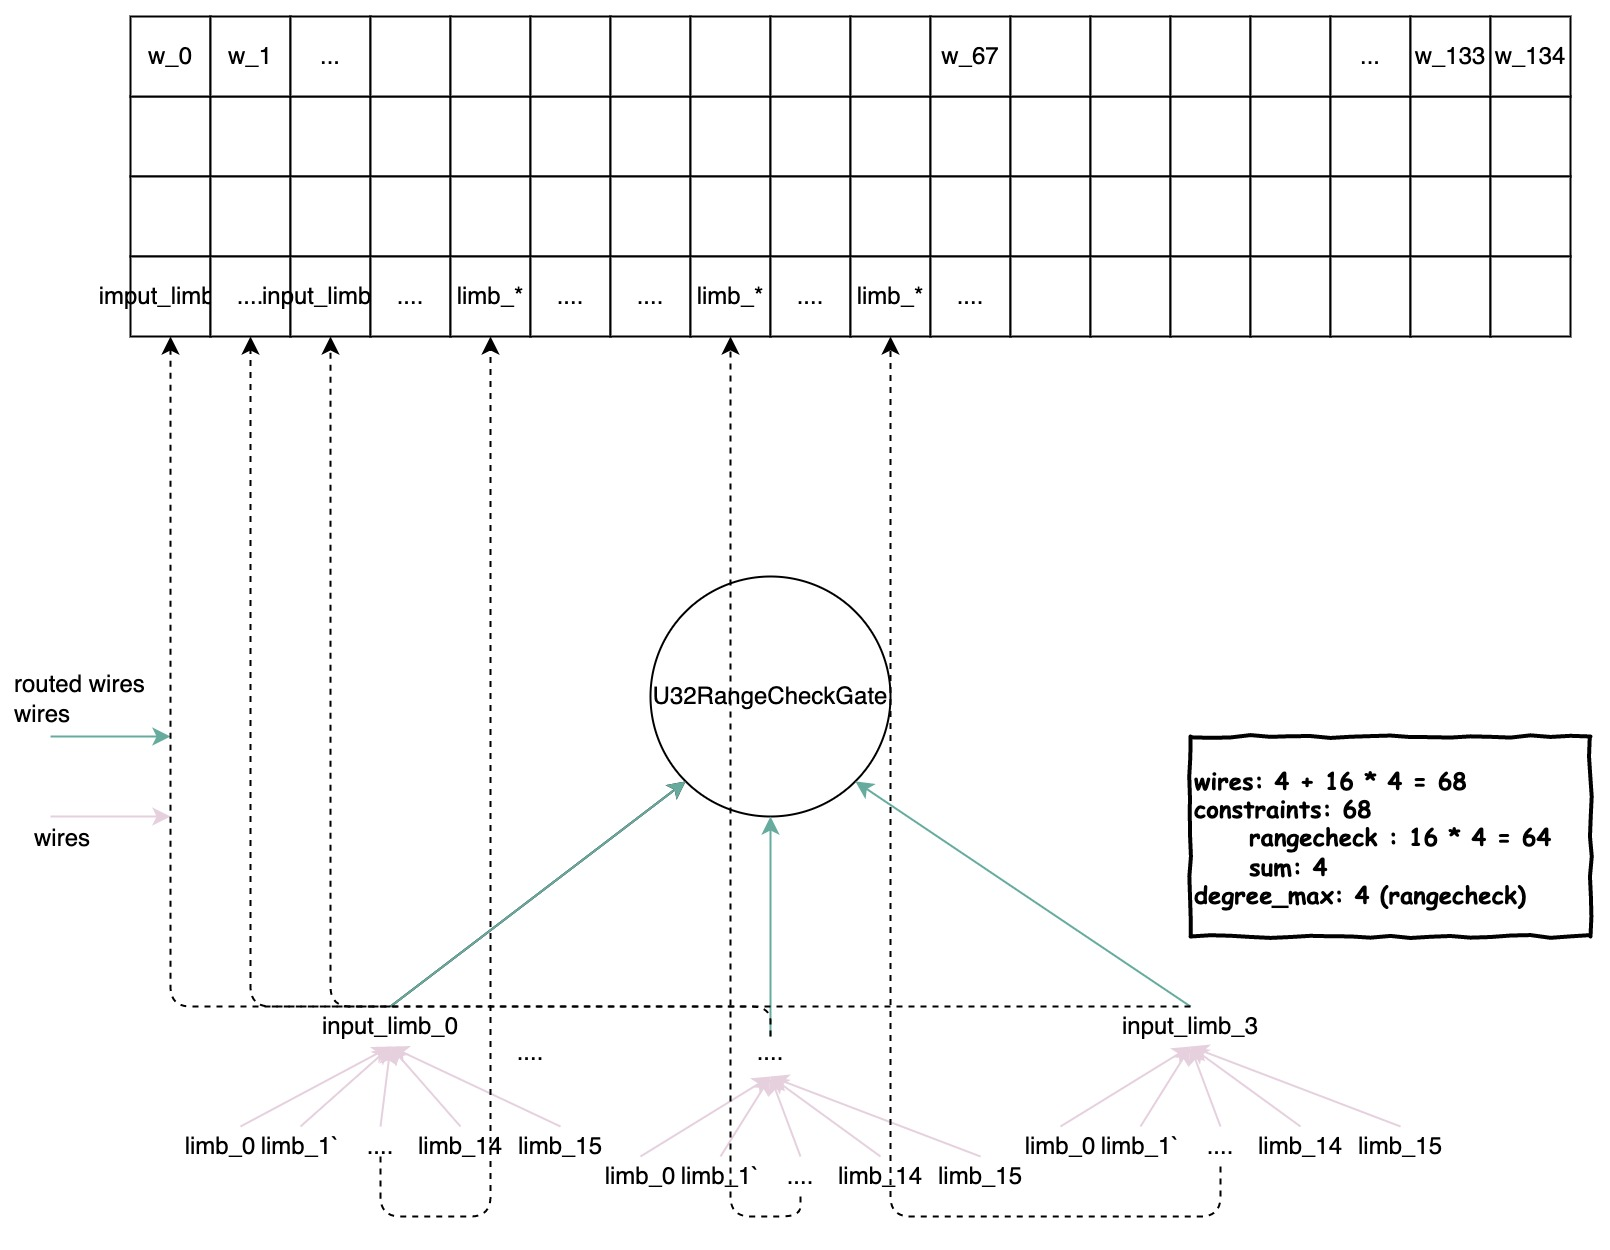
\includegraphics[width=0.8\textwidth]{gates/range_check_u32.jpeg}
    \caption{U32RangeCheckGate}
    \label{fig:range-check-u32}
\end{figure}

Constraints for each input\_limb:
\begin{itemize}
    \item Each input\_limb consists of its aux\_limbs. -- 1 constraint with degree 1.
    \begin{lstlisting}
let computed_sum = reduce_with_powers(&aux_limbs, base);
constraints.push(computed_sum - input_limb);
    \end{lstlisting}
    \item aux\_limbs range check. -- 16(aux\_limbs) constraints with degree BASE((x-0)*(x-1)*...*(x-BASE+1)).
\end{itemize}

In summary, there are 17 constraints per input limbs, a total of $num\_input\_limbs * 17$ constraints. 
Degree of the gate equals $BASE$ for range check.